\begin{frame}[plain]
  \begin{figure}
    \centering
    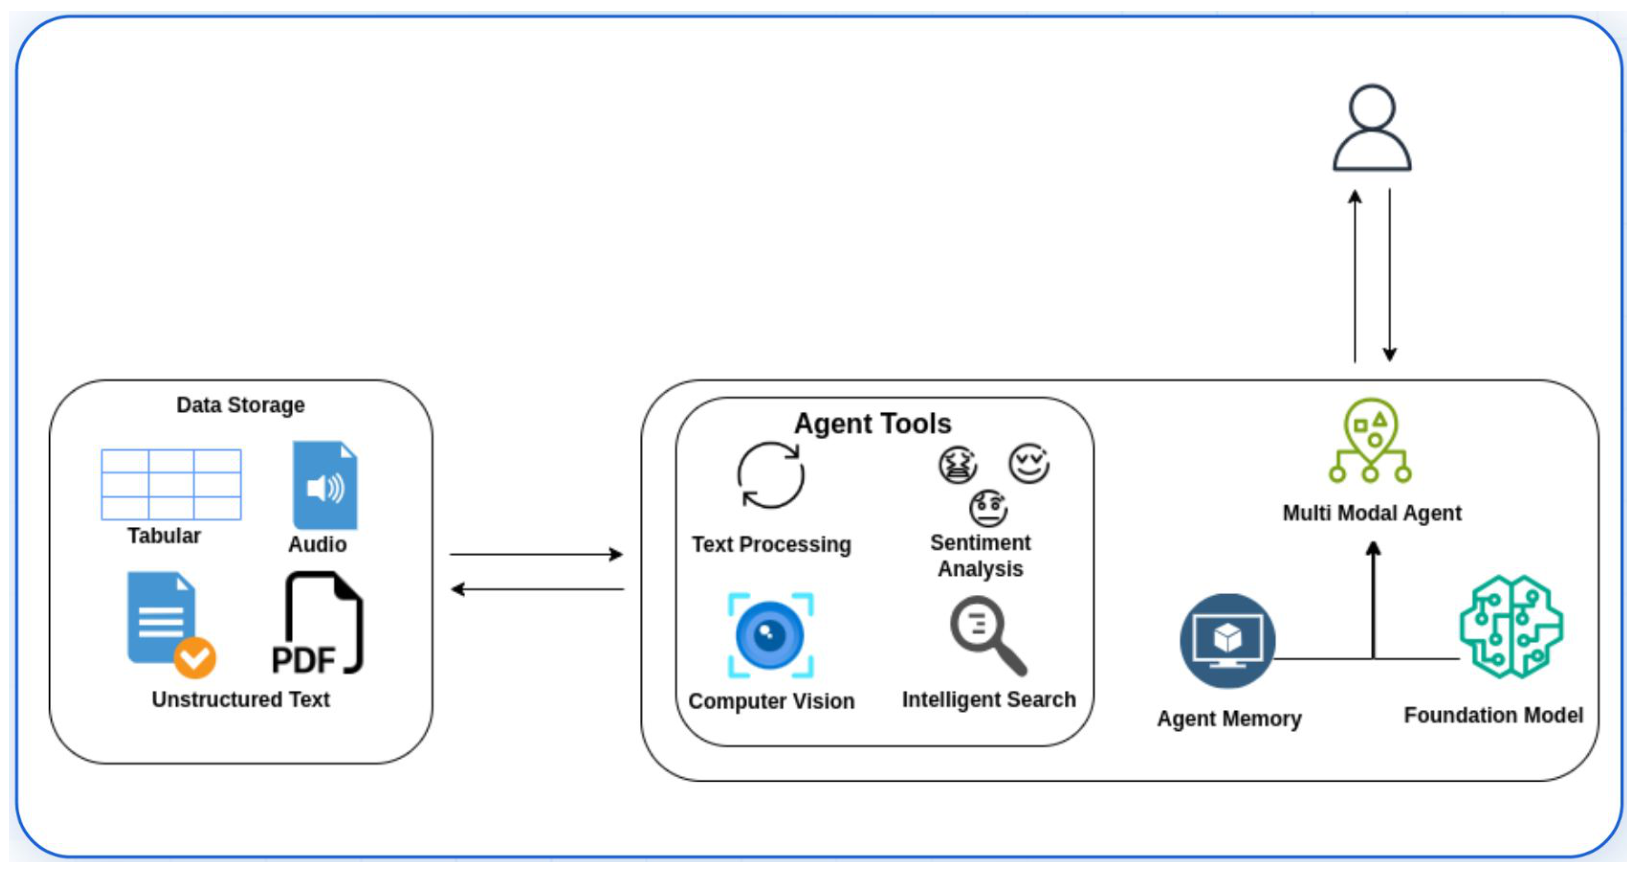
\includegraphics[width=0.8\paperwidth,height=0.74\paperheight,keepaspectratio]{images/agentic-ai/multimodal_agent_system_overview.png}
    \caption*{\scriptsize Redrawn after Nath et al., ``Generative AI and multi-modal agents in AWS: The key
    to unlocking new value in financial markets'', AWS Machine Learning Blog, 2023 (``Architecture Pattern:
    Multi-modal Agent'').}
  \end{figure}
\end{frame}

\begin{frame}{Table of Contents}
  \begin{enumerate}
    \item Motivation
    \item Learning Outcomes
    \item Agentic AI: Definitions, Reactive vs.\ Proactive Agents
    \item Agent Loop, Tool Use, and Agentic RAG
    \item Open-Source Agentic Frameworks
      \begin{enumerate}
        \item A Taxonomy of Agent Frameworks
        \item Auto-GPT and BabyAGI
        \item Other Notable Frameworks
      \end{enumerate}
  \end{enumerate}
\end{frame}

\begin{frame}{Table of Contents (contd.)}
  \begin{enumerate}
    \setcounter{enumi}{5}
    \item Code Generation
      \begin{enumerate}
        \item Benchmarks and Metrics
        \item Methods: Context, Infilling, Retrieval, Execution Feedback
        \item Representative Code LMs
      \end{enumerate}
    \item Continual Learning in Agents
    \item Safety, Ethics, and Control
    \item Future Directions
  \end{enumerate}
\end{frame}
